
%\appendix
\begin{appendices}
\chapter{Additional Classification Results}
\label{ChapterAdditionalClassificationResults}
\newpage
%Extracts from Tables \ref{SvmWindowPersonindepTable} and \ref{SvmClipPersonindepTable} were used in Tables \ref{TableAlgorithmicFeatures} and \ref{TabelHeuristicFeatures}. 
%Tables \ref{BoostWindowMultipersonTable} and \ref{SvmWindowMultipersonTable} contain additional sliding window, multi-person results and are included for completeness.


\begin{table}[H]
\centering
\caption{Adaboost, Multi-person testing, classification of sliding window examples. Mean and standard deviation performance is shown.}
\resizebox{0.6 \columnwidth}{!}{
\begin{tabular}{ c | c | c | c | c }
\hline
Test & Agree & Question & Think & Understand\\
\hline
affine & 0.62$\pm$0.09 & 0.52$\pm$0.03 & 0.53$\pm$0.06 & 0.64$\pm$0.03\\
deform-cubica & 0.51$\pm$0.11 & 0.60$\pm$0.04 & 0.57$\pm$0.03 & 0.51$\pm$0.06\\
deform-fastica & 0.51$\pm$0.11 & 0.60$\pm$0.04 & 0.57$\pm$0.03 & 0.51$\pm$0.06\\
deform-pca & 0.59$\pm$0.07 & 0.65$\pm$0.05 & 0.70$\pm$0.06 & 0.65$\pm$0.05\\
geometric-h & 0.64$\pm$0.09 & 0.69$\pm$0.04 & 0.60$\pm$0.07 & 0.65$\pm$0.05\\
geometric-a & 0.65$\pm$0.03 & 0.62$\pm$0.07 & 0.67$\pm$0.03 & 0.71$\pm$0.01\\
lbp & 0.57$\pm$0.08 & 0.67$\pm$0.03 & 0.57$\pm$0.04 & 0.59$\pm$0.04\\
lm & 0.56$\pm$0.11 & 0.66$\pm$0.03 & 0.59$\pm$0.04 & 0.46$\pm$0.05\\
\hline
affine-t & 0.62$\pm$0.09 & 0.52$\pm$0.03 & 0.53$\pm$0.06 & 0.64$\pm$0.03\\
deform-cubica-t & 0.52$\pm$0.12 & 0.60$\pm$0.04 & 0.58$\pm$0.03 & 0.51$\pm$0.06\\
deform-fastica-t & 0.46$\pm$0.13 & 0.61$\pm$0.05 & 0.58$\pm$0.03 & 0.49$\pm$0.06\\
deform-pca-t & 0.59$\pm$0.07 & 0.65$\pm$0.05 & 0.70$\pm$0.06 & 0.65$\pm$0.05\\
geometric-h-t & 0.64$\pm$0.09 & 0.69$\pm$0.04 & 0.60$\pm$0.07 & 0.65$\pm$0.05\\
lm-t & 0.56$\pm$0.11 & 0.66$\pm$0.03 & 0.60$\pm$0.03 & 0.46$\pm$0.05\\
\hline
\end{tabular}
}
\label{BoostWindowMultipersonTable}
\end{table}

\begin{table}[H]
\centering
\caption{Adaboost, Multi-person testing, classification of video clips}
\resizebox{0.6 \columnwidth}{!}{
\begin{tabular}{ c | c | c | c | c }
\hline
Test & Agree & Question & Think & Understand\\
\hline
affine & 0.59$\pm$0.08 & 0.54$\pm$0.03 & 0.51$\pm$0.03 & 0.60$\pm$0.02\\
deform-cubica & 0.50$\pm$0.11 & 0.61$\pm$0.05 & 0.59$\pm$0.02 & 0.49$\pm$0.04\\
deform-fastica & 0.50$\pm$0.11 & 0.61$\pm$0.05 & 0.59$\pm$0.02 & 0.49$\pm$0.04\\
deform-pca & 0.61$\pm$0.05 & 0.68$\pm$0.03 & 0.70$\pm$0.07 & 0.72$\pm$0.05\\
geometric-h & 0.64$\pm$0.09 & 0.71$\pm$0.04 & 0.66$\pm$0.08 & 0.69$\pm$0.04\\
geometric-a & 0.70$\pm$0.03 & 0.68$\pm$0.11 & 0.75$\pm$0.01 & 0.75$\pm$0.01\\
lbp & 0.58$\pm$0.06 & 0.68$\pm$0.04 & 0.60$\pm$0.06 & 0.62$\pm$0.05\\
lm & 0.55$\pm$0.06 & 0.65$\pm$0.02 & 0.59$\pm$0.03 & 0.46$\pm$0.05\\
\hline
affine-t & 0.59$\pm$0.08 & 0.54$\pm$0.03 & 0.53$\pm$0.05 & 0.59$\pm$0.03\\
deform-cubica-t & 0.51$\pm$0.12 & 0.61$\pm$0.05 & 0.59$\pm$0.02 & 0.49$\pm$0.04\\
deform-fastica-t & 0.45$\pm$0.14 & 0.64$\pm$0.05 & 0.60$\pm$0.00 & 0.48$\pm$0.04\\
deform-pca-t & 0.61$\pm$0.05 & 0.68$\pm$0.03 & 0.70$\pm$0.07 & 0.72$\pm$0.05\\
geometric-h-t & 0.64$\pm$0.07 & 0.71$\pm$0.04 & 0.66$\pm$0.08 & 0.69$\pm$0.03\\
lm-t & 0.55$\pm$0.06 & 0.65$\pm$0.02 & 0.60$\pm$0.02 & 0.46$\pm$0.05\\
\hline
\end{tabular}
}
\label{BoostClipMultipersonTable}
\end{table}

\begin{table}[H]
\centering
\caption{\ac{SVM}, Multi-person testing, classification of sliding window examples}
\resizebox{0.6 \columnwidth}{!}{
\begin{tabular}{ c | c | c | c | c }
\hline
Test & Agree & Question & Think & Understand\\
\hline
affine & 0.47$\pm$0.03 & 0.52$\pm$0.02 & 0.48$\pm$0.04 & 0.51$\pm$0.01\\
deform-cubica & 0.50$\pm$0.00 & 0.50$\pm$0.00 & 0.50$\pm$0.00 & 0.50$\pm$0.00\\
deform-fastica & 0.50$\pm$0.00 & 0.50$\pm$0.00 & 0.50$\pm$0.00 & 0.50$\pm$0.00\\
deform-pca & 0.50$\pm$0.02 & 0.54$\pm$0.02 & 0.53$\pm$0.03 & 0.54$\pm$0.01\\
geometric-h & 0.58$\pm$0.04 & 0.57$\pm$0.02 & 0.61$\pm$0.01 & 0.63$\pm$0.02\\
geometric-a & 0.66$\pm$0.06 & 0.67$\pm$0.05 & 0.74$\pm$0.01 & 0.73$\pm$0.03\\
lbp & 0.57$\pm$0.04 & 0.58$\pm$0.04 & 0.55$\pm$0.02 & 0.58$\pm$0.07\\
lm & 0.50$\pm$0.03 & 0.58$\pm$0.03 & 0.56$\pm$0.04 & 0.50$\pm$0.01\\
\hline
affine-t & 0.47$\pm$0.04 & 0.52$\pm$0.03 & 0.48$\pm$0.04 & 0.52$\pm$0.01\\
deform-cubica-t & 0.50$\pm$0.00 & 0.50$\pm$0.00 & 0.50$\pm$0.00 & 0.50$\pm$0.00\\
deform-fastica-t & 0.50$\pm$0.00 & 0.50$\pm$0.00 & 0.50$\pm$0.00 & 0.50$\pm$0.00\\
deform-pca-t & 0.50$\pm$0.04 & 0.61$\pm$0.03 & 0.55$\pm$0.06 & 0.54$\pm$0.02\\
geometric-h-t & 0.60$\pm$0.04 & 0.57$\pm$0.03 & 0.63$\pm$0.02 & 0.64$\pm$0.02\\
lm-t & 0.51$\pm$0.04 & 0.60$\pm$0.02 & 0.59$\pm$0.04 & 0.50$\pm$0.03\\
\hline
\end{tabular}
}
\label{SvmWindowMultipersonTable}
\end{table}

\begin{table}[H]
\centering
\caption{\ac{SVM}, Multi person testing, classification of video clips}
\resizebox{0.6 \columnwidth}{!}{
\begin{tabular}{ c | c | c | c | c }
\hline
Test & Agree & Question & Think & Understand\\
\hline
affine & 0.49$\pm$0.05 & 0.56$\pm$0.03 & 0.49$\pm$0.07 & 0.54$\pm$0.05\\
deform-cubica & 0.51$\pm$0.01 & 0.50$\pm$0.00 & 0.50$\pm$0.00 & 0.50$\pm$0.00\\
deform-fastica & 0.51$\pm$0.01 & 0.50$\pm$0.00 & 0.50$\pm$0.00 & 0.50$\pm$0.00\\
deform-pca & 0.50$\pm$0.02 & 0.61$\pm$0.02 & 0.56$\pm$0.07 & 0.49$\pm$0.03\\
geometric-h & 0.71$\pm$0.05 & 0.69$\pm$0.04 & 0.73$\pm$0.03 & 0.77$\pm$0.03\\
geometric-a & 0.70$\pm$0.06 & 0.70$\pm$0.06 & 0.83$\pm$0.01 & 0.75$\pm$0.03\\
lbp & 0.57$\pm$0.05 & 0.60$\pm$0.03 & 0.54$\pm$0.03 & 0.59$\pm$0.09\\
lm & 0.50$\pm$0.08 & 0.58$\pm$0.07 & 0.57$\pm$0.04 & 0.45$\pm$0.03\\
\hline
affine-t & 0.49$\pm$0.06 & 0.55$\pm$0.01 & 0.47$\pm$0.07 & 0.55$\pm$0.05\\
deform-cubica-t & 0.51$\pm$0.01 & 0.50$\pm$0.00 & 0.50$\pm$0.00 & 0.50$\pm$0.00\\
deform-fastica-t & 0.51$\pm$0.01 & 0.50$\pm$0.00 & 0.50$\pm$0.00 & 0.50$\pm$0.00\\
deform-pca-t & 0.55$\pm$0.02 & 0.65$\pm$0.03 & 0.57$\pm$0.06 & 0.55$\pm$0.04\\
geometric-h-t & 0.71$\pm$0.04 & 0.67$\pm$0.04 & 0.73$\pm$0.05 & 0.76$\pm$0.04\\
lm-t & 0.53$\pm$0.09 & 0.67$\pm$0.07 & 0.60$\pm$0.06 & 0.47$\pm$0.04\\
\hline
\end{tabular}
}
\label{SvmClipMultipersonTable}
\end{table}

\begin{table}[H]
\centering
\caption{Adaboost, Person independent testing, classification of sliding window examples}
\resizebox{0.6 \columnwidth}{!}{
\begin{tabular}{ c | c | c | c | c }
\hline
Test & Agree & Question & Think & Understand\\
\hline
affine & 0.61$\pm$0.02 & 0.42$\pm$0.09 & 0.50$\pm$0.03 & 0.55$\pm$0.04\\
deform-cubica & 0.55$\pm$0.07 & 0.52$\pm$0.08 & 0.55$\pm$0.06 & 0.45$\pm$0.04\\
deform-fastica & 0.55$\pm$0.07 & 0.52$\pm$0.08 & 0.55$\pm$0.06 & 0.45$\pm$0.04\\
deform-pca & 0.61$\pm$0.06 & 0.47$\pm$0.04 & 0.64$\pm$0.03 & 0.57$\pm$0.02\\
geometric-h & 0.66$\pm$0.06 & 0.61$\pm$0.06 & 0.52$\pm$0.06 & 0.56$\pm$0.06\\
geometric-a & 0.66$\pm$0.02 & 0.52$\pm$0.04 & 0.65$\pm$0.02 & 0.68$\pm$0.05\\
lbp & 0.57$\pm$0.04 & 0.53$\pm$0.13 & 0.49$\pm$0.07 & 0.44$\pm$0.05\\
lm & 0.56$\pm$0.03 & 0.54$\pm$0.10 & 0.50$\pm$0.14 & 0.41$\pm$0.04\\
\hline
affine-t & 0.62$\pm$0.02 & 0.47$\pm$0.04 & 0.49$\pm$0.03 & 0.55$\pm$0.03\\
deform-cubica-t & 0.59$\pm$0.01 & 0.56$\pm$0.06 & 0.51$\pm$0.02 & 0.47$\pm$0.01\\
deform-fastica-t & 0.55$\pm$0.07 & 0.52$\pm$0.08 & 0.55$\pm$0.06 & 0.45$\pm$0.04\\
deform-pca-t & 0.61$\pm$0.06 & 0.47$\pm$0.04 & 0.64$\pm$0.03 & 0.57$\pm$0.02\\
geometric-h-t & 0.66$\pm$0.06 & 0.61$\pm$0.06 & 0.53$\pm$0.08 & 0.56$\pm$0.06\\
lm-t & 0.57$\pm$0.03 & 0.56$\pm$0.09 & 0.50$\pm$0.14 & 0.41$\pm$0.04\\
\hline
\end{tabular}
}
\label{BoostWindowPersonindepTable}
\end{table}

\begin{table}[H]
\centering
\caption{Adaboost, Person independent testing, classification of video clips}
\resizebox{0.6 \columnwidth}{!}{
\begin{tabular}{ c | c | c | c | c }
\hline
Test & Agree & Question & Think & Understand\\
\hline
affine & 0.62$\pm$0.05 & 0.39$\pm$0.07 & 0.50$\pm$0.03 & 0.53$\pm$0.09\\
deform-cubica & 0.52$\pm$0.05 & 0.56$\pm$0.11 & 0.55$\pm$0.07 & 0.42$\pm$0.04\\
deform-fastica & 0.52$\pm$0.05 & 0.56$\pm$0.11 & 0.55$\pm$0.07 & 0.42$\pm$0.04\\
deform-pca & 0.68$\pm$0.05 & 0.50$\pm$0.09 & 0.69$\pm$0.08 & 0.60$\pm$0.04\\
geometric-h & 0.65$\pm$0.07 & 0.64$\pm$0.07 & 0.55$\pm$0.09 & 0.57$\pm$0.08\\
geometric-a & 0.70$\pm$0.03 & 0.58$\pm$0.08 & 0.74$\pm$0.03 & 0.71$\pm$0.06\\
lbp & 0.57$\pm$0.07 & 0.49$\pm$0.16 & 0.48$\pm$0.09 & 0.39$\pm$0.08\\
lm & 0.56$\pm$0.02 & 0.51$\pm$0.10 & 0.48$\pm$0.15 & 0.46$\pm$0.04\\
\hline
affine-t & 0.65$\pm$0.04 & 0.39$\pm$0.07 & 0.49$\pm$0.02 & 0.58$\pm$0.05\\
deform-cubica-t & 0.56$\pm$0.01 & 0.62$\pm$0.07 & 0.52$\pm$0.04 & 0.45$\pm$0.03\\
deform-fastica-t & 0.53$\pm$0.05 & 0.56$\pm$0.11 & 0.55$\pm$0.07 & 0.43$\pm$0.05\\
deform-pca-t & 0.68$\pm$0.05 & 0.50$\pm$0.09 & 0.69$\pm$0.08 & 0.60$\pm$0.04\\
geometric-h-t & 0.65$\pm$0.07 & 0.64$\pm$0.07 & 0.55$\pm$0.10 & 0.56$\pm$0.09\\
lm-t & 0.56$\pm$0.02 & 0.54$\pm$0.07 & 0.46$\pm$0.13 & 0.44$\pm$0.04\\
\hline
\end{tabular}
}
\label{BoostClipPersonindepTable}
\end{table}

\begin{table}[H]
\centering
\caption{\ac{SVM}, Person independent testing, classification of sliding window examples.
%\ref{TableAlgorithmicFeatures} and \ref{TabelHeuristicFeatures}.
}
\resizebox{0.6 \columnwidth}{!}{
\begin{tabular}{ c | c | c | c | c }
\hline
Test & Agree & Question & Think & Understand\\
\hline
affine & 0.49$\pm$0.03 & 0.51$\pm$0.04 & 0.45$\pm$0.04 & 0.50$\pm$0.03\\
deform-cubica & 0.50$\pm$0.00 & 0.50$\pm$0.00 & 0.50$\pm$0.00 & 0.50$\pm$0.00\\
deform-fastica & 0.50$\pm$0.00 & 0.50$\pm$0.00 & 0.50$\pm$0.00 & 0.50$\pm$0.00\\
deform-pca & 0.50$\pm$0.00 & 0.50$\pm$0.00 & 0.50$\pm$0.00 & 0.50$\pm$0.00\\
\rowcolor[gray]{.95} geometric-h & 0.59$\pm$0.02 & 0.51$\pm$0.02 & 0.52$\pm$0.02 & 0.56$\pm$0.02\\
\rowcolor[gray]{.95} geometric-a & 0.66$\pm$0.03 & 0.54$\pm$0.01 & 0.70$\pm$0.03 & 0.70$\pm$0.02\\
lbp & 0.55$\pm$0.05 & 0.51$\pm$0.11 & 0.49$\pm$0.08 & 0.47$\pm$0.08\\
lm & 0.50$\pm$0.00 & 0.51$\pm$0.01 & 0.49$\pm$0.01 & 0.51$\pm$0.00\\
\hline
affine-t & 0.49$\pm$0.03 & 0.52$\pm$0.04 & 0.46$\pm$0.04 & 0.50$\pm$0.03\\
deform-cubica-t & 0.50$\pm$0.00 & 0.50$\pm$0.00 & 0.50$\pm$0.00 & 0.50$\pm$0.00\\
deform-fastica-t & 0.50$\pm$0.00 & 0.50$\pm$0.00 & 0.50$\pm$0.00 & 0.50$\pm$0.00\\
deform-pca-t & 0.50$\pm$0.00 & 0.51$\pm$0.01 & 0.50$\pm$0.00 & 0.50$\pm$0.00\\
\rowcolor[gray]{.95} geometric-h-t & 0.60$\pm$0.02 & 0.51$\pm$0.02 & 0.55$\pm$0.02 & 0.58$\pm$0.02\\
lm-t & 0.51$\pm$0.00 & 0.51$\pm$0.01 & 0.48$\pm$0.01 & 0.50$\pm$0.01\\
\hline
\end{tabular}
}
\label{SvmWindowPersonindepTable}
\end{table}

\begin{table}[H]
\centering
\caption{\ac{SVM}, Person independent testing, classification of video clips. %\ref{TableAlgorithmicFeatures} and \ref{TabelHeuristicFeatures}.
}
\resizebox{0.6 \columnwidth}{!}{
\begin{tabular}{ c | c | c | c | c }
\hline
Test & Agree & Question & Think & Understand\\
\hline
affine & 0.53$\pm$0.05 & 0.56$\pm$0.07 & 0.48$\pm$0.02 & 0.56$\pm$0.04\\
deform-cubica & 0.50$\pm$0.00 & 0.50$\pm$0.00 & 0.50$\pm$0.00 & 0.50$\pm$0.00\\
deform-fastica & 0.50$\pm$0.00 & 0.50$\pm$0.00 & 0.50$\pm$0.00 & 0.50$\pm$0.00\\
deform-pca & 0.50$\pm$0.00 & 0.50$\pm$0.00 & 0.50$\pm$0.00 & 0.50$\pm$0.00\\
\rowcolor[gray]{.95} geometric-h & 0.73$\pm$0.04 & 0.54$\pm$0.08 & 0.58$\pm$0.00 & 0.68$\pm$0.08\\
\rowcolor[gray]{.95} geometric-a & 0.67$\pm$0.02 & 0.64$\pm$0.05 & 0.77$\pm$0.04 & 0.71$\pm$0.05\\
lbp & 0.60$\pm$0.02 & 0.51$\pm$0.12 & 0.47$\pm$0.07 & 0.49$\pm$0.06\\
lm & 0.50$\pm$0.02 & 0.50$\pm$0.03 & 0.47$\pm$0.01 & 0.49$\pm$0.01\\
\hline
affine-t & 0.55$\pm$0.04 & 0.55$\pm$0.06 & 0.49$\pm$0.03 & 0.54$\pm$0.07\\
deform-cubica-t & 0.50$\pm$0.00 & 0.50$\pm$0.00 & 0.50$\pm$0.00 & 0.50$\pm$0.00\\
deform-fastica-t & 0.50$\pm$0.00 & 0.50$\pm$0.00 & 0.50$\pm$0.00 & 0.50$\pm$0.00\\
deform-pca-t & 0.50$\pm$0.01 & 0.50$\pm$0.01 & 0.50$\pm$0.01 & 0.50$\pm$0.00\\
\rowcolor[gray]{.95} geometric-h-t & 0.74$\pm$0.03 & 0.57$\pm$0.05 & 0.60$\pm$0.02 & 0.69$\pm$0.06\\
lm-t & 0.50$\pm$0.03 & 0.50$\pm$0.06 & 0.44$\pm$0.01 & 0.47$\pm$0.03\\
\hline
\end{tabular}
}
\label{SvmClipPersonindepTable}
\end{table}

\section{Performance of NVC Using Various Backchannel Features and Classifiers}

Row averages from Tables \ref{BoostClipMultipersonReceiverTable} to \ref{SvmClipPersonindepReceiverTable} were used to generate Table \ref{TableBackchannel}.

\begin{table}[H]
\centering
\caption{Boost, multi-person testing, classification of video clips, receiver features}
\resizebox{0.6 \columnwidth}{!}{
\begin{tabular}{ c | c | c | c | c }
\hline
Test & Agree & Question & Think & Understand\\
\hline
affine & 0.46$\pm$0.10 & 0.63$\pm$0.06 & 0.53$\pm$0.07 & 0.49$\pm$0.04\\
deform-cubica & 0.44$\pm$0.06 & 0.67$\pm$0.03 & 0.51$\pm$0.02 & 0.45$\pm$0.07\\
deform-fastica & 0.44$\pm$0.06 & 0.67$\pm$0.03 & 0.51$\pm$0.02 & 0.45$\pm$0.07\\
deform-pca & 0.51$\pm$0.02 & 0.70$\pm$0.04 & 0.68$\pm$0.02 & 0.59$\pm$0.02\\
geometric-h & 0.58$\pm$0.03 & 0.69$\pm$0.01 & 0.73$\pm$0.05 & 0.62$\pm$0.04\\
geometric-a & 0.67$\pm$0.03 & 0.62$\pm$0.05 & 0.72$\pm$0.06 & 0.70$\pm$0.04\\
lbp & 0.51$\pm$0.05 & 0.69$\pm$0.04 & 0.58$\pm$0.05 & 0.54$\pm$0.01\\
lm & 0.48$\pm$0.06 & 0.68$\pm$0.04 & 0.55$\pm$0.05 & 0.51$\pm$0.09\\
\hline
affine-t & 0.46$\pm$0.10 & 0.63$\pm$0.06 & 0.52$\pm$0.06 & 0.47$\pm$0.06\\
deform-cubica-t & 0.45$\pm$0.05 & 0.67$\pm$0.03 & 0.51$\pm$0.02 & 0.47$\pm$0.07\\
deform-fastica-t & 0.45$\pm$0.05 & 0.67$\pm$0.03 & 0.51$\pm$0.02 & 0.47$\pm$0.07\\
deform-pca-t & 0.51$\pm$0.02 & 0.70$\pm$0.04 & 0.68$\pm$0.02 & 0.59$\pm$0.02\\
geometric-h-t & 0.58$\pm$0.03 & 0.69$\pm$0.01 & 0.73$\pm$0.05 & 0.61$\pm$0.04\\
lm-t & 0.48$\pm$0.06 & 0.68$\pm$0.04 & 0.55$\pm$0.05 & 0.48$\pm$0.08\\
\hline
\end{tabular}
}
\label{BoostClipMultipersonReceiverTable}
\end{table}

\begin{table}[H]
\centering
\caption{Boost, person-independent testing, classification of video clips, receiver features}
\resizebox{0.6 \columnwidth}{!}{
\begin{tabular}{ c | c | c | c | c }
\hline
Test & Agree & Question & Think & Understand\\
\hline
affine & 0.43$\pm$0.05 & 0.57$\pm$0.05 & 0.53$\pm$0.02 & 0.46$\pm$0.04\\
deform-cubica & 0.41$\pm$0.03 & 0.60$\pm$0.06 & 0.45$\pm$0.08 & 0.51$\pm$0.04\\
deform-fastica & 0.41$\pm$0.03 & 0.60$\pm$0.06 & 0.45$\pm$0.08 & 0.51$\pm$0.04\\
deform-pca & 0.48$\pm$0.02 & 0.60$\pm$0.07 & 0.47$\pm$0.04 & 0.53$\pm$0.07\\
geometric-h & 0.61$\pm$0.06 & 0.57$\pm$0.11 & 0.59$\pm$0.06 & 0.58$\pm$0.04\\
geometric-a & 0.63$\pm$0.04 & 0.43$\pm$0.04 & 0.65$\pm$0.13 & 0.64$\pm$0.06\\
lbp & 0.46$\pm$0.06 & 0.54$\pm$0.13 & 0.45$\pm$0.10 & 0.45$\pm$0.06\\
lm & 0.45$\pm$0.07 & 0.64$\pm$0.03 & 0.42$\pm$0.04 & 0.49$\pm$0.07\\
\hline
affine-t & 0.44$\pm$0.04 & 0.52$\pm$0.10 & 0.49$\pm$0.04 & 0.45$\pm$0.05\\
deform-cubica-t & 0.41$\pm$0.02 & 0.60$\pm$0.06 & 0.45$\pm$0.08 & 0.51$\pm$0.03\\
deform-fastica-t & 0.40$\pm$0.02 & 0.62$\pm$0.03 & 0.47$\pm$0.10 & 0.52$\pm$0.03\\
deform-pca-t & 0.48$\pm$0.02 & 0.60$\pm$0.07 & 0.47$\pm$0.04 & 0.53$\pm$0.07\\
geometric-h-t & 0.61$\pm$0.06 & 0.57$\pm$0.11 & 0.59$\pm$0.06 & 0.54$\pm$0.03\\
lm-t & 0.45$\pm$0.07 & 0.64$\pm$0.03 & 0.42$\pm$0.05 & 0.49$\pm$0.06\\
\hline
\end{tabular}
}
\label{BoostClipPersonindepReceiverTable}
\end{table}

\begin{table}[H]
\centering
\caption{\ac{SVM}, multi-person testing, classification of video clips, receiver features}
\resizebox{0.6 \columnwidth}{!}{
\begin{tabular}{ c | c | c | c | c }
\hline
Test & Agree & Question & Think & Understand\\
\hline
affine & 0.46$\pm$0.05 & 0.59$\pm$0.02 & 0.47$\pm$0.05 & 0.46$\pm$0.03\\
deform-cubica & 0.51$\pm$0.01 & 0.50$\pm$0.00 & 0.51$\pm$0.01 & 0.50$\pm$0.00\\
deform-fastica & 0.51$\pm$0.01 & 0.50$\pm$0.00 & 0.51$\pm$0.01 & 0.50$\pm$0.00\\
deform-pca & 0.53$\pm$0.02 & 0.59$\pm$0.04 & 0.52$\pm$0.06 & 0.51$\pm$0.02\\
geometric-h & 0.64$\pm$0.05 & 0.69$\pm$0.03 & 0.65$\pm$0.04 & 0.63$\pm$0.06\\
geometric-a & 0.67$\pm$0.04 & 0.58$\pm$0.03 & 0.72$\pm$0.04 & 0.71$\pm$0.02\\
lbp & 0.61$\pm$0.01 & 0.59$\pm$0.05 & 0.51$\pm$0.07 & 0.46$\pm$0.05\\
lm & 0.54$\pm$0.02 & 0.63$\pm$0.02 & 0.53$\pm$0.03 & 0.50$\pm$0.05\\
\hline
affine-t & 0.45$\pm$0.05 & 0.57$\pm$0.02 & 0.47$\pm$0.06 & 0.45$\pm$0.02\\
deform-cubica-t & 0.51$\pm$0.01 & 0.50$\pm$0.00 & 0.51$\pm$0.01 & 0.50$\pm$0.00\\
deform-fastica-t & 0.51$\pm$0.01 & 0.50$\pm$0.00 & 0.51$\pm$0.01 & 0.50$\pm$0.00\\
deform-pca-t & 0.52$\pm$0.03 & 0.62$\pm$0.04 & 0.55$\pm$0.05 & 0.53$\pm$0.03\\
geometric-h-t & 0.65$\pm$0.04 & 0.70$\pm$0.04 & 0.66$\pm$0.04 & 0.61$\pm$0.04\\
lm-t & 0.56$\pm$0.05 & 0.66$\pm$0.03 & 0.54$\pm$0.04 & 0.50$\pm$0.07\\
\hline
\end{tabular}
}
\label{SvmClipMultipersonReceiverTable}
\end{table}

\begin{table}[H]
\centering
\caption{\ac{SVM}, person-independent testing, classification of video clips, receiver features}
\resizebox{0.6 \columnwidth}{!}{
\begin{tabular}{ c | c | c | c | c }
\hline
Test & Agree & Question & Think & Understand\\
\hline
affine & 0.43$\pm$0.03 & 0.57$\pm$0.07 & 0.46$\pm$0.07 & 0.48$\pm$0.04\\
deform-cubica & 0.50$\pm$0.00 & 0.50$\pm$0.00 & 0.50$\pm$0.00 & 0.50$\pm$0.00\\
deform-fastica & 0.50$\pm$0.00 & 0.50$\pm$0.00 & 0.50$\pm$0.00 & 0.50$\pm$0.00\\
deform-pca & 0.50$\pm$0.00 & 0.50$\pm$0.00 & 0.50$\pm$0.00 & 0.50$\pm$0.00\\
geometric-h & 0.59$\pm$0.04 & 0.55$\pm$0.04 & 0.49$\pm$0.03 & 0.54$\pm$0.03\\
geometric-a & 0.64$\pm$0.07 & 0.43$\pm$0.06 & 0.60$\pm$0.12 & 0.67$\pm$0.06\\
lbp & 0.54$\pm$0.07 & 0.51$\pm$0.11 & 0.43$\pm$0.05 & 0.47$\pm$0.06\\
lm & 0.47$\pm$0.04 & 0.49$\pm$0.02 & 0.48$\pm$0.01 & 0.48$\pm$0.01\\
\hline
affine-t & 0.41$\pm$0.05 & 0.57$\pm$0.08 & 0.46$\pm$0.08 & 0.48$\pm$0.05\\
deform-cubica-t & 0.50$\pm$0.00 & 0.50$\pm$0.00 & 0.50$\pm$0.00 & 0.50$\pm$0.00\\
deform-fastica-t & 0.50$\pm$0.00 & 0.50$\pm$0.00 & 0.50$\pm$0.00 & 0.50$\pm$0.00\\
deform-pca-t & 0.49$\pm$0.01 & 0.50$\pm$0.01 & 0.50$\pm$0.00 & 0.50$\pm$0.01\\
geometric-h-t & 0.62$\pm$0.05 & 0.55$\pm$0.09 & 0.54$\pm$0.02 & 0.56$\pm$0.03\\
lm-t & 0.47$\pm$0.04 & 0.47$\pm$0.05 & 0.46$\pm$0.02 & 0.45$\pm$0.04\\
\hline
\end{tabular}
}
\label{SvmClipPersonindepReceiverTable}
\end{table}

\chapter{Linear Predictor Feature Tracking}
\label{BackgroundLpTracking}

Natural conversations contain wide range of head poses, which may be subject to sudden and rapid pose change. This work uses a pre-existing tracking method proposed by Ong \etal \cite{Ong2009}, called \ac{LP} feature tracking. This section introduces the theory of \ac{LP} trackers because it has not previously been applied to emotion or \ac{NVC} recognition.

\def\supportOffset{\textbf{c}}
\def\numSupportPixels{m}
\def\imageIntensityDifference{\delta \textbf{p}}
\def\imageIntensity{\textbf{V}}
\def\predictedMotion{\textbf{t}}
\def\numTrainingOffsets{h}
\def\lpTrainingIntensity{\textbf{T}}
\def\lpTrainOffsets{\delta \textbf{P}}
\def\linearPredictorMapping{\textbf{H}}
\def\numShapeComponents{r}

\begin{figure}[tb]
\centering
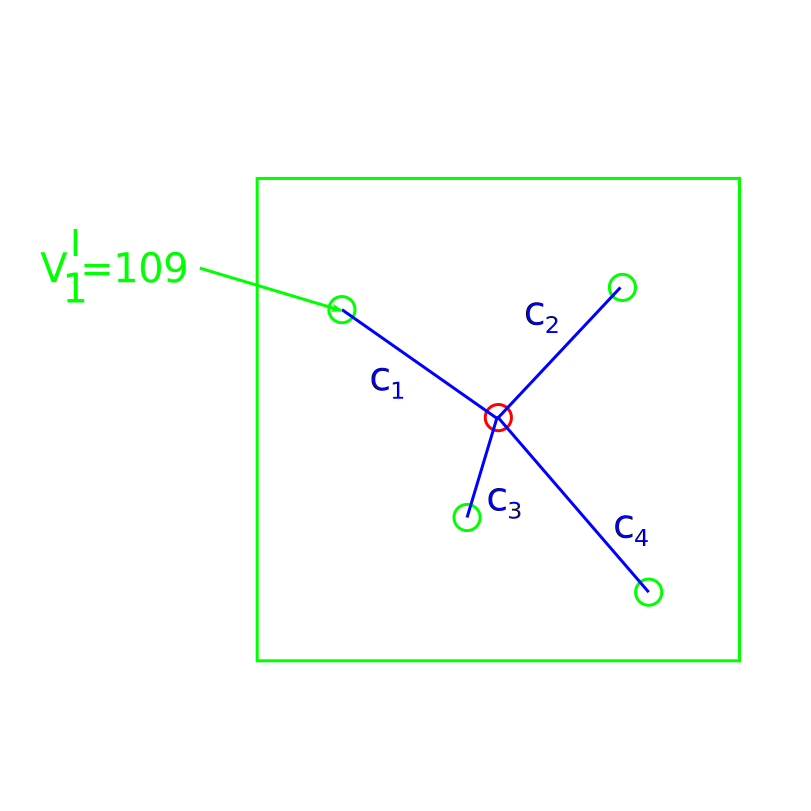
\includegraphics[width = 0.5 \columnwidth]{litreview/lptracker.pdf}
\caption[The basic structure of an LP is shown, with the position of interest marked in red.]{The basic structure of an LP is shown, with the position of interest marked in red. There are four support pixels with offsets, $\supportOffset_1$ to $\supportOffset_4$. The image intensity for support pixel 1 is shown ($\imageIntensity^I_1$). The square shows the area from which the support pixels are sampled.}
\label{FigureLinearPredictorTrain}
\end{figure}

An \ac{LP} tracker is associated with $\numSupportPixels$ ``support pixels'', where $\numSupportPixels \geq 1$. Each support pixel has a fixed 2{D} offset $\supportOffset$ from the \ac{LP} tracker position. Support pixels surrounding the \ac{LP} position is depicted in Figure \ref{FigureLinearPredictorTrain}. Also, each support pixel is assigned an initial pixel intensity at training time. Point trackers are required to predict a point of interest's motion in a series of frames. This can be expressed as the tracker providing a prediction to move from the position on the previous frame $\rawTracking^{n-1}$ to the position of interest's location on the current frame $\rawTracking^{n}$. An \ac{LP} makes the motion prediction based on the difference $\imageIntensityDifference$ between the initial support pixel intensities $\imageIntensity^I$ and the support pixel intensities on the current frame $\imageIntensity$. Typically, images are converted to grey-scale, since the hue of the face is approximately uniform and therefore not useful for tracking. The predicted motion from the previous frame to the current frame $\predictedMotion$ is a simple linear mapping $\linearPredictorMapping$:

\begin{gather}
\label{LinearPredictionMapping}
\predictedMotion = \linearPredictorMapping \imageIntensityDifference \\
\label{LinearPredictionIntensity}
\imageIntensityDifference = \imageIntensity - \imageIntensity^I
\end{gather}

\begin{figure}[tb]
\centering
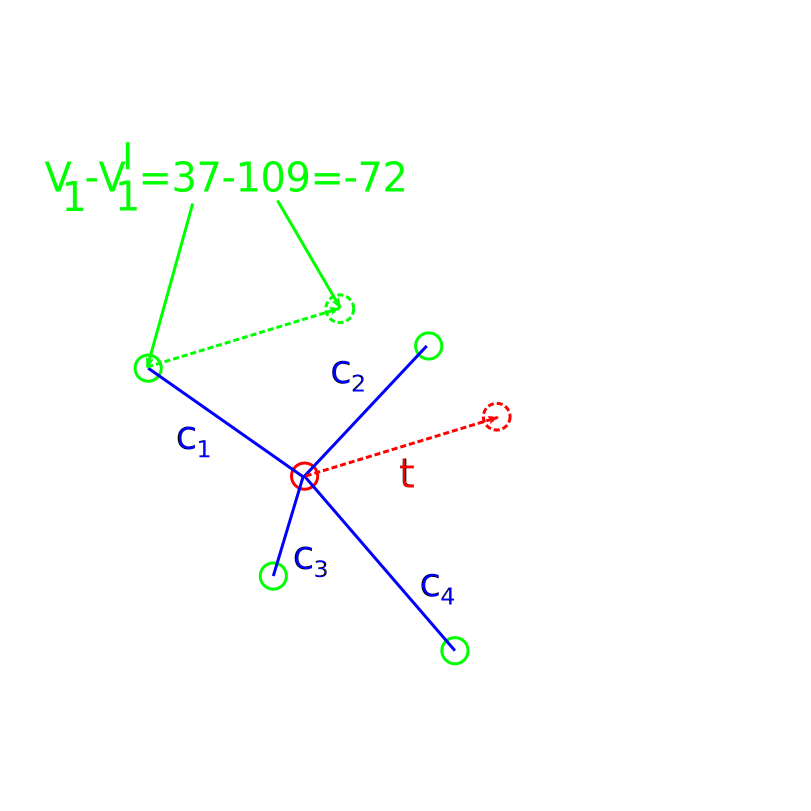
\includegraphics[width = 0.5 \columnwidth]{litreview/lptracker2.pdf}
\caption[The \ac{LP} is offset by $\predictedMotion$, which results in changes in intensity for all the support pixels.]{The \ac{LP} is offset by $\predictedMotion$, which results in changes in intensity for all the support pixels. The intensity change for support pixel 1 is shown. The object of linear predictors is to find a linear mapping $\linearPredictorMapping$ between position offset and the change in support pixel intensities.}
\label{FigureLinearPredictorOffset}
\end{figure}

Training an \ac{LP} is based on one or more frames in which the position of interest has been manually specified. Multiple frames are used because it enables the \ac{LP} tracker to generalise to multiple head poses. $\numSupportPixels$ support pixel offsets are uniformly sampled from a square centred on the tracker position. The initial support pixel intensities $\imageIntensity^I$ are set to the average pixel intensity of the support pixel locations in the training frames. Training examples are generated synthetically, based on offset the tracker by a known offset $\predictedMotion$ and storing the pixel intensity differences at the offset position. Many synthetic offsets can be generated for each training frame, resulting in $\numTrainingOffsets$. The training intensity differences stored in a matrix $\lpTrainingIntensity$ of size $\numTrainingOffsets$ by $\numSupportPixels$. The training offset matrix $\lpTrainOffsets$ is of size $\numTrainingOffsets$ by $2$. The mapping $\linearPredictorMapping$ can be found by taking the pseudo-inverse of the training intensities.

\begin{gather}
\linearPredictorMapping = \lpTrainOffsets \lpTrainingIntensity^{+}
\end{gather}

Applying \ac{LP}s to an unseen sequence involves finding the pixel intensities $\imageIntensity$ at the current tracker position and applying equations \ref{LinearPredictionMapping} and \ref{LinearPredictionIntensity} to find the predicted motion.

One common failure mode of the tracking is for a single tracker to drift, while the others track correctly. These errors can often be corrected by using shape constraints, which restrict face deformations to be similar to previously observed configurations. This was a common technique that provides the basis for \ac{ASM}s \cite{Cootes1992}. The technique is applied by learning a PCA shape model from the training frames and then modifying the feature tracking procedure, so each frame is processed as follows:

\begin{enumerate}
 \item track new frame based on position from previous frame,
 \item project tracking positions into PCA space,
 \item retain the first $\numShapeComponents$ eigenvalues and discard the rest,
 \item reconstruct the tracking positions, then
 \item perform tracking as further refinement, starting at the reconstructed tracker positions.
\end{enumerate}

The number of eigenvalues to retain $\numShapeComponents$ is normally selected to preserve 90\% (or some other manually specified proportion) of the variation of the training data.

Section \ref{SectionLpTracking} describes how this method is applied to \ac{NVC} classification.

\chapter{Photograph Permissions}
\label{AppendixPhotoPermissions}

Photos used in Figure \ref{FigureManualGestureNvc}:

``Waving goodbye after the ceremony'' \copyright Jonathan Elderfield, \newline
https://secure.flickr.com/photos/heatheranneulrich/3420075962/ \newline
Used by permission, under the terms of the Creative Commons Attribution-NonCommercial-NoDerivs 2.0 Generic License \newline
https://creativecommons.org/licenses/by-nc-nd/2.0/

``Bank of America security trying to prevent me from taking a photo during the Iraq war protest'' \copyright Steve Rhodes \newline
https://secure.flickr.com/photos/ari/2347593532/ \newline
Used by permission, under the terms of the Creative Commons Attribution-NonCommercial-ShareAlike 2.0 Generic License \newline
https://creativecommons.org/licenses/by-nc-sa/2.0/

Photos used in Figure \ref{FigureGazeNvc}:

``Eye contact'' \copyright Jessie Reeder \newline
https://secure.flickr.com/photos/elizacole/2503079623/ \newline
Used by permission, under the terms of the Creative Commons Attribution-NonCommercial-NoDerivs 2.0 Generic License \newline
https://creativecommons.org/licenses/by-nc-nd/2.0/

``Wink'' \copyright Dave77459 \newline
https://secure.flickr.com/photos/dave77459/3083102723/ \newline
Used by permission, under the terms of the Creative Commons Attribution-NonCommercial-ShareAlike 2.0 Generic License \newline
https://creativecommons.org/licenses/by-nc-sa/2.0/

\chapter{Questionnaire}
\label{ChapterQuestionnaire}

\Large
Rate Communication Signals in Human Conversation

\large
Instructions

\normalsize 
View the video sequences with audio turn on and answer the following questions.

Videos are displayed in this page (for your convenience) if you use a browser that supports the latest video standards (Firefox 3.5, etc) or Flash.

Does this person disagree or agree with what is being said?(required)

\includegraphics[width = 0.9 \columnwidth]{corpus/questionagree.png}

A score of 5 is neutral or not applicable.

Is this person thinking hard?(required)

\includegraphics[width = 0.9 \columnwidth]{corpus/questionthinking.png}

Is this person asking a question?(required)

\includegraphics[width = 0.9 \columnwidth]{corpus/questionquestion.png}

Is this person indicating they understand what is being said to them?(required)

\includegraphics[width = 0.9 \columnwidth]{corpus/questionunderstand.png}

\chapter{Behaviour Mimicry and Pearson's Correlation}
\label{ChapterMimicryColleration}

Section \ref{SectionMirrorBehaviour} describes a method for automatically identifying some types of behaviour including some types of synchrony and mimicry. Detecting behaviour by comparing simulations frames recorded on two cameras of two different subjects may seem counter intuitive because mimicry occurs in response to another behaviour. Although it is true that samples are paired in terms of observation time, the correlation coefficient is based on the overall video. This allows coupled variations to be identified, particularly if they are slowly varying.

A simple synthetic illustrative example of mimicry will now be discussed to demonstrate that Pearson's correlation is sensitive to mimicry in this case. Imagine two people in conversation with their behaviours being monitored. Assume we have a single behaviour measure for each person; what this represents is totally arbitrary but it could be some measure of body pose or facial expression. In a simple case, one person repeatedly changes behaviour and the other person mimics this after a time delay. For simplicity, person A changes their behaviour at 1Hz (the period is 0.5Hz). The time delay of person B's mimicked behaviour to be 0.3 sec. Of course, most behaviours are not this regular or rapid but this is just a simple illustration of the principle. The variation of the behaviour is shown in Figure \ref{FigureMimicryCorellation}.

\begin{figure}
\centering
\includegraphics[width = 0.80 \columnwidth]{conclusion/mimicry-pearsons.png}

\caption[Synthetic example of mimicry]{A synthetic example of mimicry: person A changes their behaviour at 1Hz (the period is 0.5Hz). The time delay of person B's mimicked behaviour is 0.3 sec.}
\label{FigureMimicryCorellation}
\end{figure}

When using the method proposed in Section \ref{SectionMirrorBehaviour}, the Pearson correlation of these two components is 0.46. This demonstrates that for this type of mimicry, the method can find measurable linear coupling between these two variables. As long as there is some overlap in behaviours, the approach is sensitive and therefore suitable. This method is not suitable for certain types of rapid behaviours. For example, if blinking was coupled, this approach would not be suitable because the behaviour of Person A would likely have ended before Person B would have started to mimic it.

\end{appendices}